\section{Approach}
\label{sec:approach}

\begin{figure*}[t]
\centering
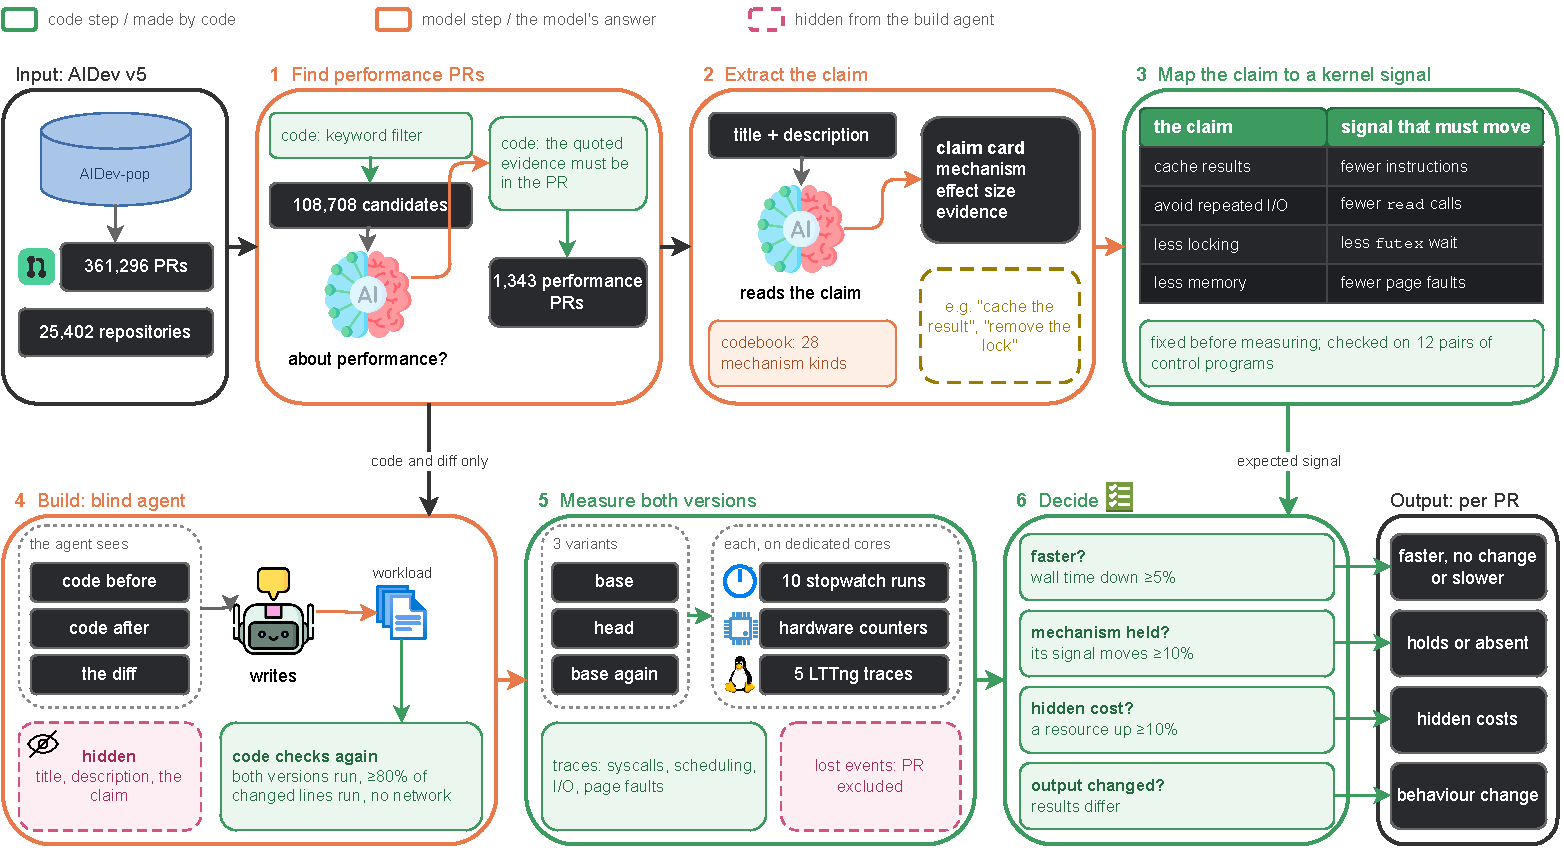
\includegraphics[width=\textwidth]{figures/final.pdf}
\caption{Overview of \sys. Orange boxes are model steps and green boxes
are code. The build agent (step~4) sees only the code and the diff; the
PR text and the claim are hidden from it (pink). The expected signal from
step~3 goes straight to the decision in step~6.}
\label{fig:overview}
\end{figure*}

Figure~\ref{fig:overview} shows the six steps of the pipeline.

\subsection{Performance PRs and their claims}
\label{sec:data}
We use AIDev~\cite{li2026aidev} (version~5, pinned to one dataset commit),
restricted to its \emph{AIDev-pop} subset of \nPop agent PRs from
\nPopRepos repositories with more than 100 stars. A keyword filter over
titles, bodies and commit messages (after removing per-agent template
text) keeps \nCand candidates (\pctCand). An LLM classifier with a written
codebook labels whether a PR's goal is to make the software run faster or
use fewer resources; on a random sample of \nPilot candidates,
\pctPilotRuntime are runtime-performance PRs and \pctPilotNone are not
about performance at all. A stratified run over candidates that change
Python code (fixed random order per agent, with a stop rule per agent)
classifies \nStratClassified PRs and yields \nRuntimePRs runtime-performance
PRs. Labels come from Claude Opus~5.5 (\nStratOpus PRs) and, to save cost,
Claude Haiku~5.5 (\nStratHaiku PRs); on \haikuAgreeN PRs labelled by both,
they agree on \haikuAgree (Cohen's $\kappa=\haikuKappa$). Every label
must quote its evidence verbatim from the PR; code checks the quote.

A second codebook, revised once after open coding of 100 PRs and then
frozen, extracts from each runtime-performance PR the mechanism(s) it
claims (28 categories), the claimed effect size, and the evidence it
offers (Table~\ref{tab:oracle} lists the measurable mechanisms).

\subsection{From claimed mechanism to kernel signal}
\label{sec:oracle}
Each mechanism is mapped, before any measurement, to the signals that must
move if the claim is true (Table~\ref{tab:oracle}). Twelve pairs of small
control programs, one pair per signal family, show that each signal moves
as designed: e.g.\ reading a file 2,000 times instead of once, or a
two-thread mutex against per-thread counters.

\begin{table}[t]
\caption{Claimed mechanism, share of the \nClaims runtime-performance PRs
that claim it (a PR may claim several), and the signal that must move.}
\label{tab:oracle}
\centering\scriptsize
\setlength{\tabcolsep}{3pt}
\begin{tabular}{@{}lrl@{}}
\toprule
mechanism claimed & PRs & signal (head vs.\ base) \\
\midrule
skip unneeded work & \mechSkipUnneededWork & fewer syscalls / instructions \\
less memory, fewer copies & \mechLessMemory & fewer page faults, page allocations \\
cache results & \mechCacheResults & fewer instructions (and syscalls) \\
algorithmic & \mechAlgorithmic & fewer instructions, syscalls unchanged \\
parallelize & \mechParallelize & wall time down, CPU time not down \\
async / non-blocking I/O & \mechAsyncIo & less off-CPU time on the main thread \\
precompute & \mechPrecompute & fewer instructions on the hot path \\
faster library & \mechFasterLibrary & fewer instructions \\
concurrency tuning & \mechConcurrencyTuning & threads, context switches, futex \\
lazy loading & \mechLazyLoading & fewer \texttt{openat} / bytes read \\
reuse resources & \mechReuseResources & fewer \texttt{socket}/\texttt{connect}/\texttt{clone} \\
DB: faster / fewer queries & \mechFasterDbQuery\,/\,\mechFewerDbQueries & fewer page reads, round trips \\
vectorize, locality & \mechVectorizeLocality & fewer instructions, cache misses \\
avoid repeated I/O & \mechAvoidRepeatedIo & fewer \texttt{openat}/\texttt{read}, bytes \\
less locking & \mechLessLocking & less futex wait \\
\bottomrule
\end{tabular}
\end{table}

\subsection{Blind build agent and measurement}
\label{sec:harness}
For each PR, the harness checks out the merge base and the PR head (the
API's base commit can be later than the branch point and would mix in
unrelated changes), installs both with dependencies frozen at the PR's
creation date, and hands them to a build agent (Claude Code, Opus~5.5).
The agent is \emph{blind to the claim}: it sees the code, the diff and the
changed files, but not the title, description, commit messages or our
extracted claim, and the git history is moved out of its reach. It must
write a deterministic workload that runs the changed code on both
versions, may stub only external I/O, and must not patch the code under
test. The harness then re-checks independently: both versions run, the
workload executes at least 80\% of the executable lines the PR adds or
changes (50\% for PRs with over 200 such lines), the base version runs 0.5--30\,s, the
workload runs without a network, and the two output digests are compared.
Transcripts are audited for access to the PR on GitHub.

Measurements run on \nVMs identical Google Cloud C4 virtual machines with
the performance-monitoring unit enabled, one job per machine at a time.
Workloads run on dedicated cores (one, or two for parallel workloads):
system services are confined to the other cores with systemd, because \texttt{isolcpus} disables load balancing
(a two-process pool ran on a single core). Per PR we run base, head and
base again (an A/A control): 3+3 warm-up runs, 10 untraced timing runs per
variant, 5 runs of 3 hardware-counter groups (at most four programmable
events each, so no counter is multiplexed), and 5 full LTTng kernel traces
per variant (all syscalls, scheduling, block I/O, interrupts, page faults,
page allocation), filtered to the workload's process tree and with per-file
I/O attribution. PRs with any lost trace events or multiplexed counters are excluded from
the analysis. On each machine,
the \nControls control pairs pass \ctrlPassMin--\ctrlPassMax of \nChecks
checks; the only failure is context switches under lock contention, a
non-deterministic signal whose primary signal (\texttt{futex}) passes. An
exact-instruction loop is counted within a relative error of
$\counterErrMax$, and LTTng's page-fault events agree with perf's fault
counter at a median ratio of \faultRatioMed.
